\documentclass[11pt]{article}

%Menge: \mathbb{R}

\usepackage[ngerman]{babel}
\usepackage{amsmath} %align, f¸r = untereinander einfach &=
\usepackage{amssymb}
\usepackage{amsthm}
\graphicspath{ {./images/} }
\usepackage{listings}
\usepackage[utf8]{inputenc}
\usepackage{graphicx}
\usepackage[left=1.80cm, right=1.80cm, top=1.30cm, bottom=2.00cm]{geometry}

%eigene Befehle:
\newcommand{\R}{$\mathbb{R}$}


\title{Blatt 6} %% Template in den entsprechenden Namen ändern


\begin{document}
\lstset{language=Java}
\author{Tom Herrmann}
\date{\today}
\maketitle
\section{Aufgabe 2}
\subsection{a}
\begin{center}
	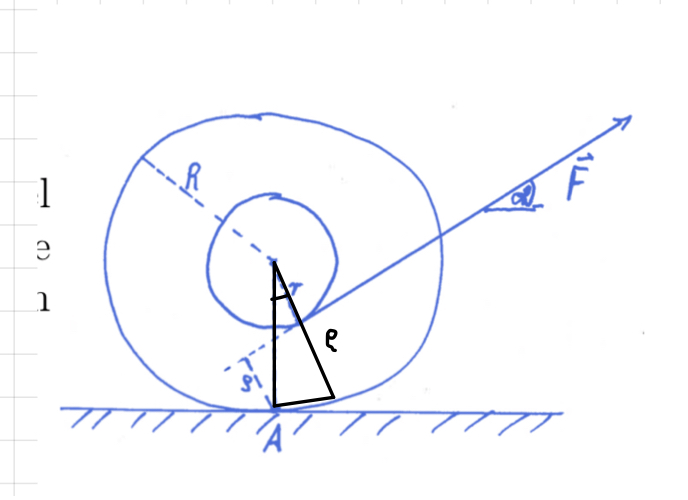
\includegraphics[scale= 0.5]{IMG_E710CED3176C-1.jpeg}
\end{center}
Aus dem eingezeichneten Dreieck kann man die Beziehung direkt ablesen und ist damit recht offensichtlich.
\subsection{b}
\begin{align*}
	cos \alpha ? \frac{r + \rho}{R}\\
	-\vec{M} = \vec{r} \tiems \vec{F} \qquad |\vec{M}| = |\vec{r}| |\vec{F}| sin \varphi\\
	M = \rho \cdot F = 0\\
	
\end{align*}

\end{document}




